\documentclass[../main.tex]{subfiles}
\begin{document}

\chapter{Methodology} % (fold)
\label{cha:methodology}

\section{Database description} % (fold)
\label{sec:database_description}

% \begin{figure}[h]
% \centering
% 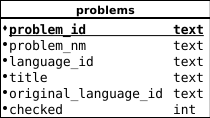
\includegraphics{img/db/problems}
% % \includesvg{img/db/problems}
% \decoRule
% \caption[An Electron]{An electron (artist's impression).}
% \label{fig:Electron}
% \end{figure}

Here is the list of the table in the database:

% \begin{itemize}
% 	\item abstractproblems
% 	\item compilers
% 	\item courses
% 	\item courseslists
% 	\item coursesusers
% 	\item listitems
% 	\item lists
% 	\item problems
% 	\item problemstags
% 	\item submissions
% 	\item users
% \end{itemize}

\subsection{users} % (fold)
\label{sub:users}

\fboxsep=0mm%padding thickness
\fboxrule=2pt%border thickness

\begin{wrapfigure}{l}{0.33\textwidth}
  \vspace{-20pt}
  \begin{center}
    \fcolorbox{black}{black}{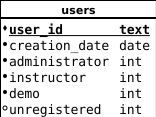
\includegraphics[width=0.31\textwidth]{img/db/users}}
  \end{center}
  \vspace{-20pt}
  % \caption{A gull}
  % \vspace{-10pt}
\end{wrapfigure}

\paragraph{Description:}~\\ % (fold)
The first table contains the users. For this analysis, the user table has been anonymized. We only refer to a user ID, and his contributions in the data base. Personal data from users will not be used for analysis. Only the creation date is kept for a time based analysis.  

However, it's needed to exclude some \emph{non-representative} users :

\begin{itemize}
	\setlength\itemsep{0em}
	\item Some users used for developement ([list])
	\item Users with a id patern different that \emph{Uxxxxx} (Users used for competition for exemple)
	\item Demonstrations users ($demo == 1 $).
	\item Instructors, administrators and unregistred users (cf flags atributes in the database).
\end{itemize}

\paragraph{Numbers:}~\\ % (fold)
In term of numbers, the database contains:
\begin{itemize}
	\setlength\itemsep{0em}
	\item 10565 users in total.
	\item 55 unregistred users.
	\item 50 instructors.
	\item 7 administrators.
	\item 1 demo user.
\end{itemize}

% subsection users (end)

\newpage
\subsection{problems and abstractproblems} % (fold)
\label{sub:problems}
\begin{wrapfigure}{l}{0.45\textwidth}
  \vspace{-20pt}
  \begin{center}
    \fcolorbox{black}{black}{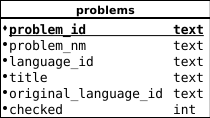
\includegraphics[width=0.42\textwidth]{img/db/problems}}
  \end{center}
  \vspace{-10pt}
  % \caption{A gull}
  % \vspace{-10pt}
\end{wrapfigure}

\paragraph{Description:}~\\ % (fold)
A single problem could be proposed in various languages but the language variation doesn't affect the technical details of a same problem. That means that the way how a submission would be processed is never linked to the language\footnote{There are actually few problems which differ between languages for inputs or outputs regarding to the language but those are negligible}.

\begin{wrapfigure}{r}{0.3\textwidth}
  \vspace{-20pt}
  \begin{center}
    \fcolorbox{black}{black}{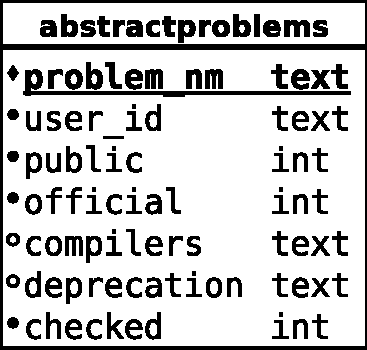
\includegraphics[width=0.28\textwidth]{img/db/abstractproblems}}
  \end{center}
  \vspace{-20pt}
  % \caption{A gull}
  % \vspace{-10pt}
\end{wrapfigure}

That explains those two tables discribing the problems. The first one colled \emph{abstractproblems} contains the technical informations for submission management. The second one, \emph{problems}, is the description of a problem, according to a specific language (\emph{language\_id}) and refering to a \emph{abstractproblems}.

There is different types of problems :
\begin{itemize}
	\setlength\itemsep{0em}
	\item \emph{Pxxxxx}\\
	Those type of problems will be our baseline for the analysis. In fact, they are the \emph{offical} problems initialy present in the database, created by the designers. We can consider them as \emph{right} and \emph{relevant} in term of submission and veredict\footnote{The concept of veredict will be explain in the following section \emph{submissions table}}.

	\item \emph{Xxxxxx}\\
	The letter \emph{X} means \emph{externe}. Those problems have been created by users (\emph{instructors}) and havn't been validatd by anyone. Moreover, only a portion of users can acces to it (Those who suscribed to the courses related to the same instructor)

	\item \emph{Gxxxxx}\\
	The letter \emph{G} means \emph{game}. Those problems are used on a very specific scenario. There is only a very few of them and they will be ignored in our analysis.

	\item \emph{deprecated}\\
	Obviously, this type of problem is not relevant for the analysis. 

\end{itemize}

\paragraph{Numbers:}%~\\ % (fold)
\begin{itemize}
	\setlength\itemsep{0em}
	\item 1909 abstractproblems in total.
	\item 1325 Pxxxxx like abstractproblems.
	\item 575 Xxxxxx like abstractproblems.
	\item 9 Gxxxxx like abstractproblems.
	\item 85 deprecated abstractproblems (including 21 Pxxxx type). 
\end{itemize}

\newpage
\subsection{submissions} % (fold)
\label{sub:submissions}

\begin{wrapfigure}{l}{0.58\textwidth}
  \vspace{-20pt}
  \begin{center}
    \fcolorbox{black}{black}{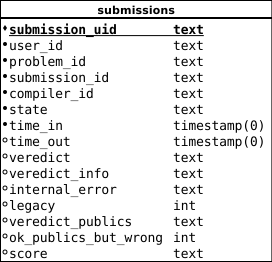
\includegraphics[width=0.54\textwidth]{img/db/submissions}}
  \end{center}
  \vspace{-20pt}
  % \caption{A gull}
  % \vspace{-10pt}
\end{wrapfigure}

\paragraph{Description:}~\\ % (fold)
Every instance in this table represents the submission of a solution for a specific problem (\emph{problem\_id}) by a specific user (\emph{user\_id}) at a given time/moment (\emph{time\_in (time\_out)}). Form that submission (after a internal process) will stand out a veredict meaningful of the submission correctness.

\paragraph{Numbers:}%~\\ % (fold)
\begin{itemize}
	\item 
	\item 
	\item 
\end{itemize}


\paragraph{Veredict distribution :} % (fold)

\begin{center}
\begin{tabular}{lcr}
\toprule
 Acronym &               Veredict &     \% \\
\midrule
      AC &               Accepted &   43.62 \\
      WA &           Wrong Answer &   30.06 \\
      EE &        Execution Error &   11.41 \\
      CE &      Compilation Error &   10.70 \\
      PE &     Presentation Error &    3.62 \\
      SC &                 Scored &    0.30 \\
      IC &      Invalid Character &    0.29 \\
      SE &           Setter Error &    0.01 \\
      FE &           Fatal Errors &    0.00 \\
      NC &  Noncompliant Solution &    0.00 \\
 Pending &     Pending Submission &    0.00 \\
      IE &         Internal Error &    0.00 \\
\bottomrule
\end{tabular}
\end{center}

\begin{figure}[h]
\centering
\fcolorbox{black}{white}{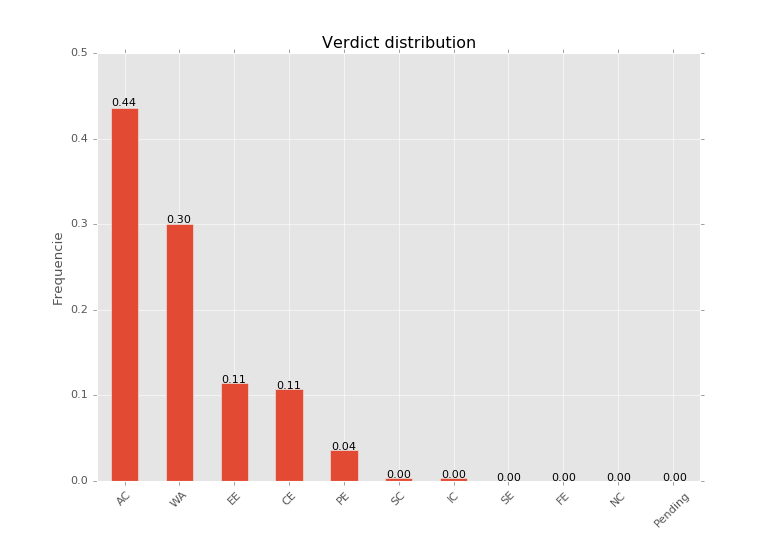
\includegraphics[width=\textwidth]{img/db/veredict_distrib}}
% \decoRule
\caption[Veredict distribution]{Frequency distribustion of veredict accros every relevant submissions}
\label{fig:veredict_distrib}
\end{figure}

% subsubsection veredict_distribution (end)

% \lipsum[2-3]

% subsection submissions (end)

% subsection problems (end)


\subsection{courseslists} % (fold)
\label{sub:courseslists}

\begin{wrapfigure}{l}{0.27\textwidth}
  \vspace{-20pt}
  \begin{center}
    \fcolorbox{black}{black}{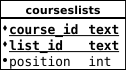
\includegraphics[width=0.25\textwidth]{img/db/courseslists}}
  \end{center}
  \vspace{-20pt}
  % \caption{A gull}
  % \vspace{-10pt}
\end{wrapfigure}

\lipsum[2-3]

% subsection courseslists (end)

\newpage
\subsection{courses} % (fold)
\label{sub:courses}

\begin{wrapfigure}{l}{0.38\textwidth}
  \vspace{-20pt}
  \begin{center}
    \fcolorbox{black}{black}{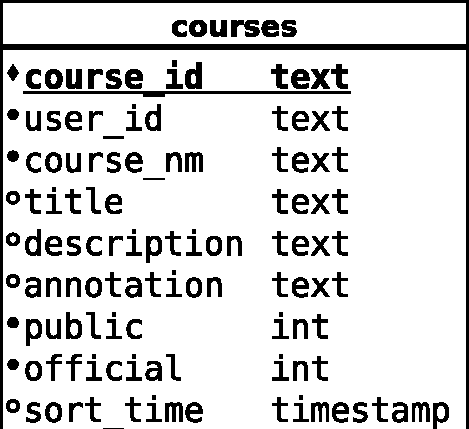
\includegraphics[width=0.36\textwidth]{img/db/courses}}
  \end{center}
  \vspace{-20pt}
  % \caption{A gull}
  % \vspace{-10pt}
\end{wrapfigure}

\lipsum[2-3]

% subsection courses (end)

\subsection{coursesusers} % (fold)
\label{sub:coursesusers}

\begin{wrapfigure}{l}{0.27\textwidth}
  \vspace{-20pt}
  \begin{center}
    \fcolorbox{black}{black}{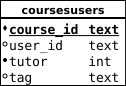
\includegraphics[width=0.25\textwidth]{img/db/coursesusers}}
  \end{center}
  \vspace{-20pt}
  % \caption{A gull}
  % \vspace{-10pt}
\end{wrapfigure}

\lipsum[2-3]

% subsection coursesusers (end)

\subsection{listitems} % (fold)
\label{sub:listitems}

\begin{wrapfigure}{l}{0.3\textwidth}
  \vspace{-20pt}
  \begin{center}
    \fcolorbox{black}{black}{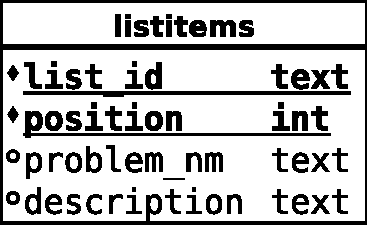
\includegraphics[width=0.28\textwidth]{img/db/listitems}}
  \end{center}
  \vspace{-20pt}
  % \caption{A gull}
  % \vspace{-10pt}
\end{wrapfigure}

\lipsum[2-3]

% subsection listitems (end)

\subsection{lists} % (fold)
\label{sub:lists}

\begin{wrapfigure}{l}{0.38\textwidth}
  \vspace{-20pt}
  \begin{center}
    \fcolorbox{black}{black}{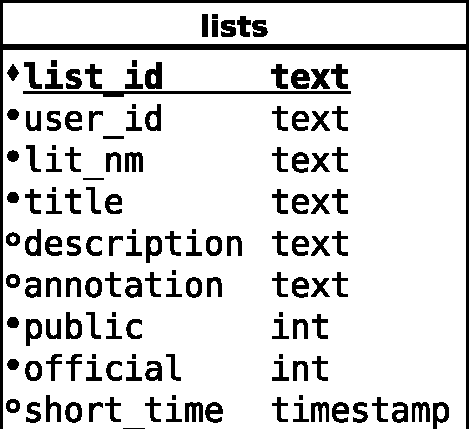
\includegraphics[width=0.36\textwidth]{img/db/lists}}
  \end{center}
  \vspace{-20pt}
  % \caption{A gull}
  % \vspace{-10pt}
\end{wrapfigure}

\lipsum[2-3]

% subsection lists (end)


\subsection{problemstags} % (fold)
\label{sub:problemstags}

\begin{wrapfigure}{l}{0.28\textwidth}
  \vspace{-20pt}
  \begin{center}
    \fcolorbox{black}{black}{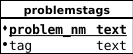
\includegraphics[width=0.26\textwidth]{img/db/problemstags}}
  \end{center}
  \vspace{-20pt}
  % \caption{A gull}
  % \vspace{-10pt}
\end{wrapfigure}

\lipsum[2-3]

% subsection problemstags (end)


% section database_description (end)
% chapter methodology (end)

\end{document}